\section{Results}

\begin{figure}[t]
    \centering
    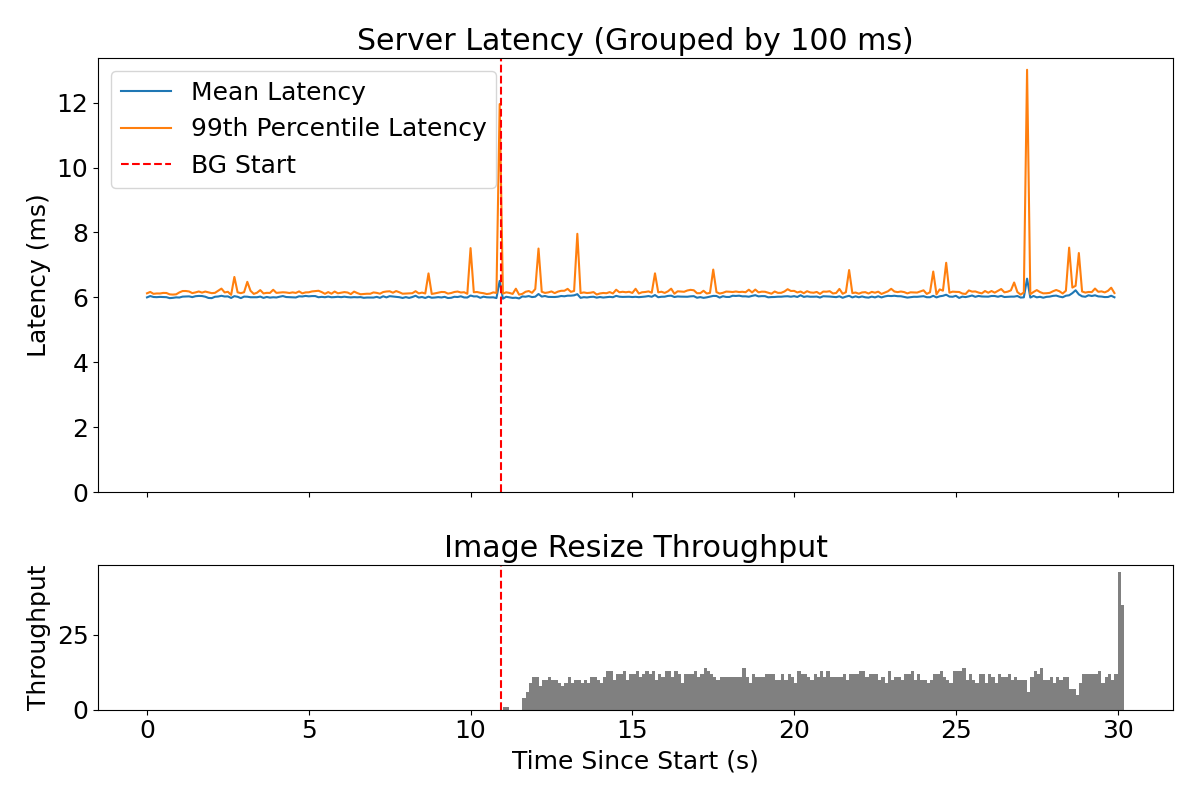
\includegraphics[width=\columnwidth]{graphs/srv-bg-schedbe-low.png}
    \caption{ \beclass{} isolates the server's latencies from BE
     jobs}\label{fig:srv-bg-schedbe}
\end{figure}
% \beclass{} isolates the server's latencies from BE
%      jobs

We re-run the microbenchmark using \beclass{}; the results are in
\autoref{fig:srv-bg-schedbe}. As desired, the latency of the server remains
stable after the BE starts, and the BE runs only in gaps where cores would
otherwise be idle.

\begin{figure}[t]
    \centering
    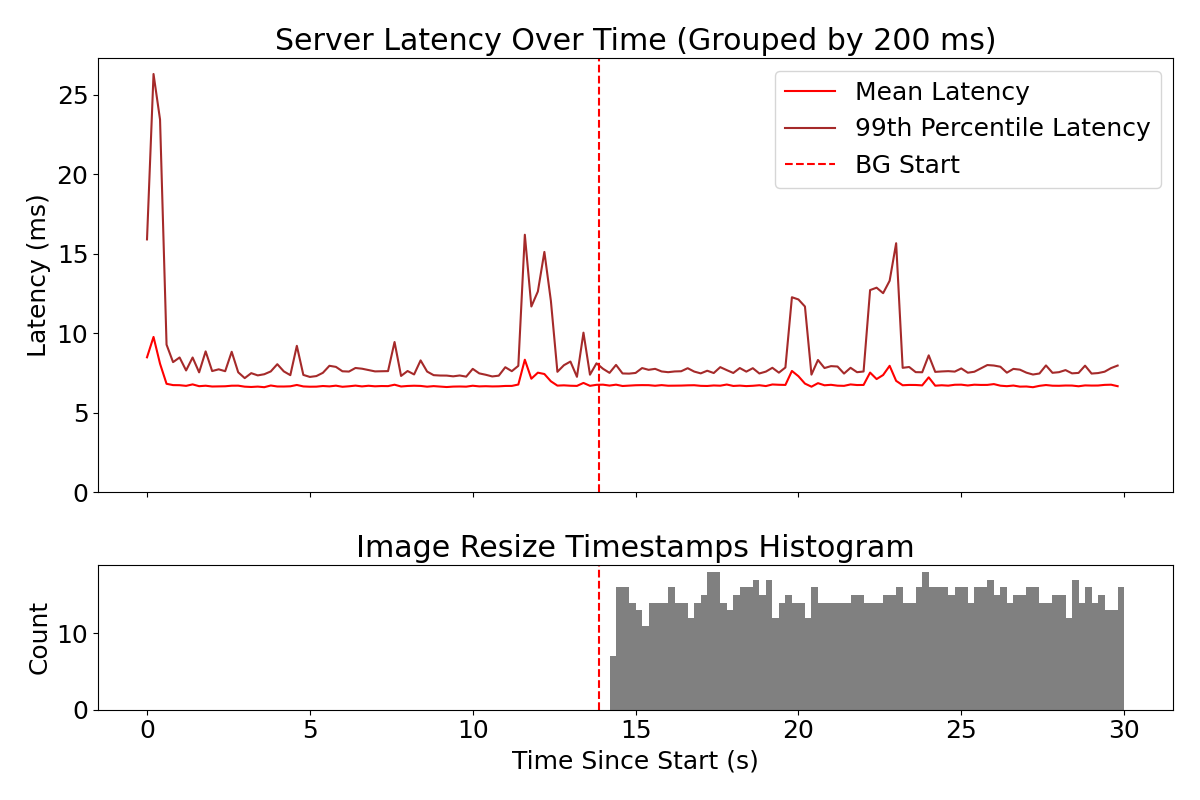
\includegraphics[width=\columnwidth]{graphs/kubernetes-schedbe.png}
    \caption{ Kubernetes using \beclass{} honors reservations, unlike in
    \autoref{fig:kubernetes-unedited} }\label{fig:kubernetes-schedbe}
\end{figure}
% Kubernetes using \beclass{} honors reservations, unlike in
%     \autoref{fig:kubernetes-unedited}

We run the Kubernetes application using \beclass{}.
\autoref{fig:kubernetes-schedbe} shows that the baseline mean latency of the LC
server stays around 6.5ms after starting the the BE.

\begin{figure}[t]
    \centering
    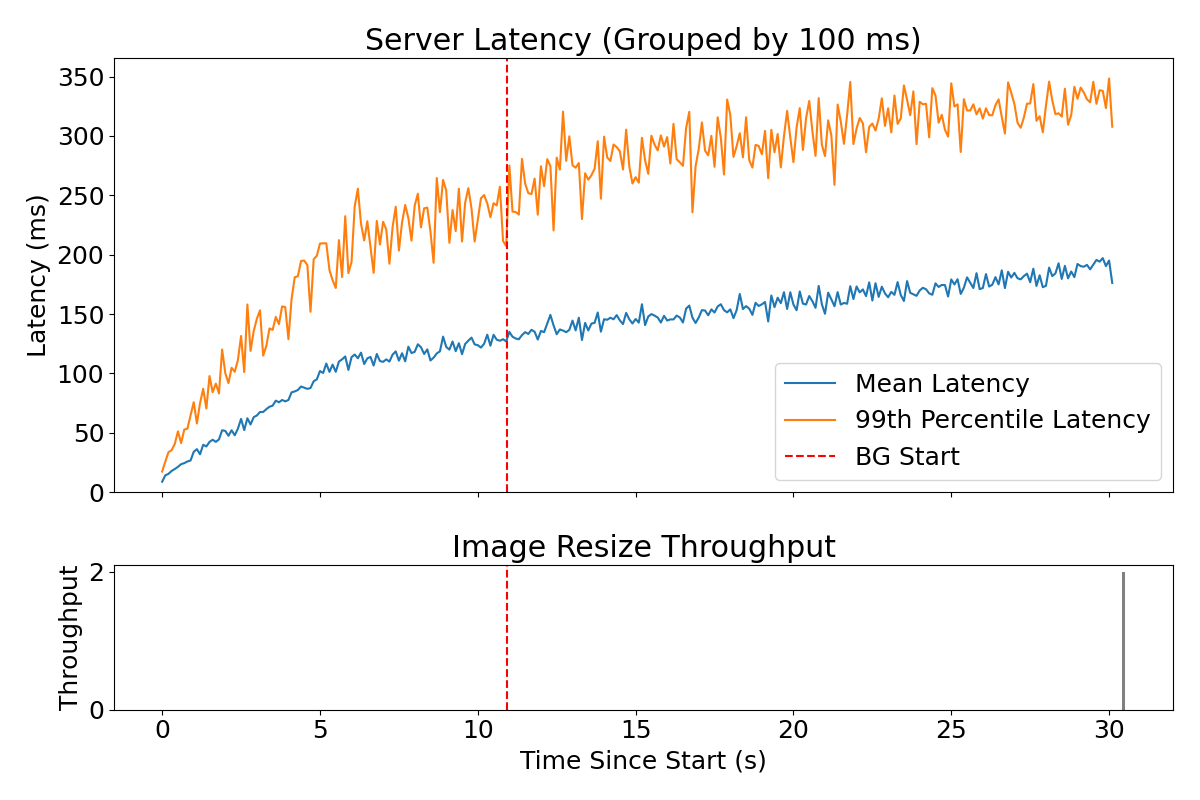
\includegraphics[width=\columnwidth]{graphs/overload-schedbe.png}
    \caption{ \beclass{} starves BE user-space threads, leaving all CPU-time to
    the LC}\label{fig:overload-schedbe}
\end{figure}
% \beclass{} starves BE user-space threads, leaving all CPU-time to
%     the LC

\autoref{fig:overload-schedbe} shows parking enables the server to keep its
reservation even under sustained 100\% load. We run the same client load as
\autoref{fig:overload-rt}, with \beclass{} parking the BE. Notice that the BE
does not make progress until the end, when the server is done processing.
